
\documentclass{aastex63}

\newcommand{\be}{\begin{eqnarray}}
\newcommand{\ee}{\end{eqnarray}}
\def\la{\mathbin{\lower 3pt\hbox
      {$\rlap{\raise 5pt\hbox{$\char'074$}}\mathchar"7218$}}}
\def\ga{\mathbin{\lower 3pt\hbox
      {$\rlap{\raise 5pt\hbox{$\char'076$}}\mathchar"7218$}}} %> or of order
\renewcommand{\vec}[1]{\mathbf{#1}}
%\renewcommand{\vec}[1]{\ensuremath{\boldsymbol{#1}}} %boldface vector style
\newcommand{\grad}{\mathbf{\nabla}}

\received{}
\revised{}
\accepted{\today}
\submitjournal{APJ}


\shorttitle{Lyman $\alpha$}
\shortauthors{uva lyman alpha group}

\graphicspath{{./}{figures/}}


\begin{document}

\title{Resonant Scattering in a Uniform Sphere with Large Optical Depth}



\correspondingauthor{Phil Arras}
\email{arras@virginia.edu}

\author{uva lyman alpha group}
%\author{Phil Arras}
%\author{Shane Davis}
\affiliation{Department of Astronomy, University of Virginia, Charlottesville, VA 22904, USA}


\begin{abstract}

The solution of the radiative transfer equation for resonant scattering of Lyman $\alpha$ photons for a uniform sphere of constant gas density is found in the limit of large line center optical depth. A monochromatic source of photons is assumed at the center of the sphere, and the intensity within the sphere and at the surface is found with the Eddington approximation for the angular dependence. The solution can be represented a sum of three terms: a simple, analytic solution of the inhomogeneous equation which diverges at the center of the sphere and at the emission frequency; a semi-analytic solution of the homogeneous equation which is required for the mean intensity $J=0$ at the surface; and finally, a solution of the homogeneous equation which enforces the correct, zero ingoing intensity boundary conditions at the surface. It is the compact, analytic form as well as the piece accounting for the correct, frequency dependent boundary condition that is novel in this study. The analytic solution is compared to numerical solutions with the Monte-Carlo method, which are valid at arbitrary optical depth, and the deviations from exact solution are investigated.

\end{abstract}


\keywords{}



ccc\section{Introduction} 
\label{sec:intro}

Nice summary paragraph from recent Bourier  papers.

Hubble Space Telescope observations have found large Lyman $\alpha$ transit depths around the gas giants HD 209458b \citep{2003Natur.422..143V}, HD 189733b \citep{2012A&A...543L...4L} and 55 Cnc b \citep{2012A&A...547A..18E}, Neptune-size planets GJ 436 b 
\citep{2015Natur.522..459E}
%, 2017A&A...605L...7L,2019A&A...629A..47D}   
and GJ 3470 b \citep{2018A&A...620A.147B}, and possibly the super-Earth HD 219134b \citep{2019EPSC...13.1928L}.
Non-detections or marginal detections have been reported for the super-Earths 55 Cnc e \citep{2012A&A...547A..18E}, super-Earth HD 97658 b \citep{2017A&A...597A..26B} , super-Earth GJ 1132 b \citep{2019AJ....158...50W}, super-Earth $\pi$ Men c \citep{2020ApJ...888L..21G}, and marginal detections were  Earth-size TRAPPIST-1 \citep{2017A&A...599L...3B} and sub-Earth Kepler-444 \citep{2017A&A...602A.106B}.


\section{ previous analytic work }

\citet{1973MNRAS.162...43H, 1974MNRAS.166..373H} started work on analytic solutions as you get a Laplace equation. Doesn't get boundary condition right.
\citet{1990ApJ...350..216N} has analytic solutions following Harrington.
\citet{1990ApJ...350..216N} improved on Harrington. Does have divergent inhomogeneous solution in slab geometry! Also has discussion of absorption.
\citet{2006ApJ...649...14D} generalized Harrington to spherical geometry
\citet{1976ApJ...208..286W} tries to compute the radiation force
\citet{1994ApJ...427..603R} discuss an ansatz for the fokker-planck approximation where the full voigt profile is used.
\citet{2020arXiv200509692L} discusses solutions for the sphere. Follows \citet{2006ApJ...649...14D}. They cite \citet{2015MNRAS.449.4336S} on core skipping.
\citet{2002ApJ...567..922A,2015MNRAS.449.4336S} discusses acceleration.
\citet{2015MNRAS.449.4336S}: amounts to drawing the atom velocity from a truncated Gaussian distribution to force it back into the wing.  The logic seems to be that almost all of the core scattering results in zero spatial diffusion until you get far enough from the line wing.  It seems like this is just calibrated by modifying the truncation until the spectrum doesn’t seem to depend sensitively on the choice of truncation.  


\section{ no photon destruction }
\label{sec:no_destruction}

Three solutions will be considered for this problem. A ``divergent" solution due to the delta function source, a ``J=0" solution which includes the delta function solution at the source and satisfies $J=0$ at $r=R$, and the ``bc" solution that allows the boundary conditions to be satisfied. The divergent solution is discussed for qualitative understanding, and the full solution is the sum of the $J=0$ solution and the bc solution.

The problem is as follows. Consider a sphere of radius $R$ and uniform density, with line-center optical depth $\tau_0 = (k/\sqrt{\pi}\Delta)R$. The transfer Equation \ref{eq:finaleqn} with no photon destruction terms, $p=\alpha_{\rm abs}=0$, and with a  photon emission term given by Equation \ref{eq:jem}), which gives the transfer equation
\be
\nabla^2 J + \left( \frac{k}{\Delta} \right)^2 \frac{\partial^2 J}{\partial \sigma^2} & = & 
- \frac{ \sqrt{6} kL}{4\pi \Delta^2} \delta^3(\vec{x} - \vec{x}_s) \delta (\sigma - \sigma_{\rm s})
\label{eq:rt_no_destr}
\ee
where the form of the source term is in Equation \ref{eq:jem_v2}. The boundary condition is no incoming flux at the surface, which can be written
\citep{1986rpa..book.....R}
\be
J & = & \sqrt{3} H
\label{eq:bc}
\ee
at $r=R$.


First consider the divergent solution. In terms of the dimensionless variables $x_1 = k(x-x_{\rm s})/\Delta$, $x_2=k(y-y_{\rm s})/\Delta$, $x_3=k(z-z_{\rm s})/\Delta$ and $x_4=\sigma - \sigma_{\rm s}$, this equation can be written as a Laplacian in the 4-dimensional space as
\be
\nabla_4^2 J & = & - \frac{\sqrt{6} k^2 L}{4\pi \Delta^3} \delta^4(x).
\ee
In terms of the 4-dimensional radius $r_4 = \sqrt{ (k/\Delta)^2\left[ (x-x_{\rm s})^2 + (y-y_{\rm s})^2 + (z-z_{\rm s})^2 \right] + (\sigma - \sigma_{\rm s})^2 }$, and assuming spherical symmetry about the source point, the equation becomes
\be
\frac{1}{r_4^3} \frac{\partial}{\partial r_4} \left( r_4^3 \frac{\partial J}{\partial r_4} \right) & = & - \frac{\sqrt{6} k^2 L}{4\pi \Delta^3} 
\frac{\delta(r_4)}{2\pi^2 r_4^3},
\ee
where the forms of the 4-dimensional Laplacian and delta function have been inserted. The ``divergent" solution due to the delta function is then
\be
J_{\rm d} & = & 
\frac{(\sqrt{6}k^2L)/(16\pi^3 \Delta^3)}{ (k/\Delta)^2\left[ (x-x_{\rm s})^2 + (y-y_{\rm s})^2 + (z-z_{\rm s})^2 \right] + (\sigma - \sigma_{\rm s})^2}.
\label{eq:Jd}
\ee
While this solution does not satisfy the surface boundary condition (Equation \ref{eq:bc}), it is accurate near the delta-function source.
This solution generalizes the particular solution for slab geometry found by \citet{1990ApJ...350..216N}. Henceforth we will focus on the source at the center of the sphere, although we will retain the emission frequency at $\sigma=\sigma_{\rm s}$. The radial flux corresponding to Equation \ref{eq:Jd} is
\be
H_{\rm d} & = & - \frac{1}{3k\phi} \frac{\partial J_d}{\partial r}
=  \left( \frac{1}{3k\phi} \right) 
\left( \frac{ \sqrt{6}k^3L }{ 8\pi^3 \Delta^4} \right)
\left( \frac{k r/\Delta}{ \left[ (kr/\Delta)^2 + (\sigma-\sigma_{\rm s})^2 \right]^2 } \right).
\label{eq:Hd}
\ee
It will be shown that Equation \ref{eq:Hd} is a good approximation at $r=R$ near line center. However Equation \ref{eq:Jd} is not a good approximation to the true solution, as it is too large at $r=R$ by a factor of $J_{\rm d}(R,\sigma)/ H_{\rm d}(R,\sigma) \sim a\tau_0/x^2 \sim (a\tau_0)^{1/3} \gg 1$. 

A better approximation to the true solution has been derived by \citet{2006ApJ...649...14D}, who generalized the closed-form solution in slab geometry found in \citet{1990ApJ...350..216N}. They found a closed-form solution which satisfies a $J=0$ boundary condition at $r=R$. We generalize their solution to allow emission at frequency $\nu_{\rm s}$ away from line center. The result is
\be
J_0 & = & \left( \frac{\sqrt{6}L}{32\pi^2 \Delta} \right)
\left( \frac{1}{Rr} \right)
\left( 
\frac{ \sin(\pi r/R) }{ \cosh \left[ \frac{\pi \Delta}{k R} (\sigma - \sigma_{\rm s}) \right] - \cos(\pi r/R)}
\right)
\label{eq:J0}
\ee
and
\be
H_0 & = & \left( \frac{1}{3k\phi} \right)
\left( \frac{\sqrt{6}L}{32\pi^2 \Delta} \right)
\left( \frac{1}{Rr^2} \right)
\left( 
\frac{ \sin(\pi r/R) }{ \cosh \left[ \frac{\pi \Delta}{k R} (\sigma - \sigma_{\rm s}) \right] - \cos(\pi r/R)}
\right. \nonumber \\ & & \left. - \left( \frac{\pi r}{R} \right)
\frac{ \cos(\pi r/R) }{ \cosh \left[ \frac{\pi \Delta}{k R} (\sigma - \sigma_{\rm s}) \right] - \cos(\pi r/R)}
+ \left( \frac{\pi r}{R} \right)
\frac{ \sin^2(\pi r/R) }{ \left[ \cosh \left[ \frac{\pi \Delta}{k R} (\sigma - \sigma_{\rm s}) \right] - \cos(\pi r/R) \right]^2 }
\right).
\label{eq:H0}
\ee
Again $J_0 \gg H_0$, except very near the $r=R$, where it goes to zero. The flux at $r=R$ can be written
\be
H_0(R,\nu) & = & \left( \frac{1}{3k\phi} \right)
\left( \frac{\sqrt{6}L}{32\pi \Delta} \right)
\left( \frac{1}{R^3} \right)
\left( 
\frac{ 1 }{ \cosh \left[ \frac{\pi \Delta}{k R} (\sigma - \sigma_{\rm s}) \right] +1 }
\right).
\label{eq:H0surf}
\ee
Equation \ref{eq:H0surf} will be shown to be a much better approximation to the solution, which is valid near the delta function at the center, and is a much better approximation at the surface. It will be shown that it is still only a good approximation near line center at the surface. It decreases exponentially rather than as a power-law in frequency, giving a much smaller flux on the line wings as compared to $H_{\rm d}$. 

The question is how to satisfy the surface boundary condition in Equation \ref{eq:bc}. On this point, we note that the derivation in \citet{1973MNRAS.162...43H}, and numerous studies later studies, does not actually produce a valid solution of the transfer equation and boundary condition. The reason is as follows. In the notation of \citet{1973MNRAS.162...43H}, a separation of variables
$J(\tau,\sigma) = \theta(\tau) j(\sigma)$ in spatial variable $\tau$ and frequency variable $\sigma$ is attempted (his Equations 16 and 23). The solutions for the eigenfunctions $\theta(\tau)$ and $j(\sigma)$ then depend explicitly on the separation constant $\lambda$. In order to satisfy the boundary conditions, the separation constant must satisfy an eigenvalue equation of the form
\be
\lambda \tan(\lambda B) & = & \frac{3}{2} \phi,
\label{eq:evalue}
\ee
where $2B$ is the slab optical depth at line center, and $\phi$ is the line profile ($\Delta \phi$ here). The key point is that the line profile depends on one of the coordinates, frequency, and this causes the eigenvalues of the separation constant to depend on frequency. But then the separation constant is not constant, and it does not satisfy Equation \ref{eq:rt_no_destr} since the frequency derivatives will will act on the separation ``constant", giving extra terms. To our knowledge the errors introduced by this ansatz have never been quantified. 

In the limit of large optical depth $B$, \citealt{1973MNRAS.162...43H} approximates the eigenvalues as $\lambda_n B \simeq \pi (n-1/2)$, which gives $J=0$ at the surface. This is essentially the result in Equation \ref{eq:J0} above. However, since this solution gives zero at the surface, his Equation 34 subsequently allowed the separation constant to have a small deviation from the above expression, which was explicitly frequency dependent. This allowed a nonzero intensity at the surface, but at the cost of rendering the separation of variables assumption invalid.

A different solution method is attempted here, namely a continuous Fourier expansion in the frequency variable $\sigma$. The full solution is written
\be
J(r,\nu) & = & J_0(r,\nu) + J_{\rm bc}(r,\nu)
\ee
and
\be
H(r,\nu) & = & H_0(r,\nu) + H_{\rm bc}(r,\nu).
\ee
Here $J_0$ and $H_0$ are the solutions of the inhomogeneous equation including the delta function source given in Equations \ref{eq:J0} and \ref{eq:H0}. The additional term $J_{\rm bc}$ must then be a solution of the homogeneous equation
\be
\frac{\partial^2J}{\partial r^2} + \frac{2}{r} \frac{\partial J}{\partial r}
+ \left( \frac{k}{\Delta} \right)^2 \frac{\partial^2 J}{\partial \sigma^2} &= & 0
\ee
with no delta function source term, and it must allow the boundary conditions to be satisfied at the surface. Since $J_0(R,
\nu)=0$, the surface boundary condition becomes
\be
J_{\rm bc}(R,\nu) - \sqrt{3} H_{\rm bc}(R,\nu) & = & 
J_{\rm bc}(R,\nu) + \frac{1}{\sqrt{3}k\phi} \frac{\partial J_{\rm bc}(R,\nu)}{\partial r} = 
\sqrt{3} H_0(R,\nu).
\label{eq:bc2}
\ee
Plugging in a frequency dependence $J \propto e^{is\sigma}$, for ``wavenumber" $s$, gives the equation for modified spherical Bessel functions of the first kind, $i_0(z)=\sinh(z)/z$. The solution can then be represented as
\be
J_{\rm bc}(r,\nu) & = & 
\int_{-\infty}^\infty \frac{ds}{2\pi} e^{is\sigma} A(s) 
\frac{i_0(krs/\Delta)}{i_0(kRs/\Delta)},
\label{eq:Jbc}
\ee
where $A(s)$ is the Fourier amplitude.

Plugging Equation \ref{eq:Jbc} into Equation \ref{eq:bc2} leads to the following equation for the Fourier amplitudes
\be
\int_{-\infty}^\infty \frac{ds}{2\pi} e^{is\sigma} A(s)
\left[ 1 + \left( \frac{s}{\sqrt{3} \Delta \phi} \right) \left( \frac{i_0^\prime(kRs/\Delta)}{i_0(kRs/\Delta)} \right) \right]
& = & \sqrt{3} H_0(R,\nu)
\label{eq:bc3}
\ee
where $H_0(R,\nu)$ is given by Equation \ref{eq:H0surf}. Discretization of Equation \ref{eq:bc3} for frequency variables $\sigma_i$ and wavenumbers $s_j$
leads to a set of coupled linear equations for the $A(s_j)$. We use equally space points $\Delta \sigma = 2\sigma_{\rm max}/(N-1)$ and $\Delta s = 2\pi/(N\Delta \sigma)$, where $N$ is the number of points for each grid. The maximum frequency is set as $\sigma_{\rm max} = {\rm constant} \times \tau_0$, for a large enough constant that  the end of the frequency grid is at such small intensities that it does not affect the solution except close to the boundaries. The number of points was increased until the solution was well-resolved near line center, and only became inaccurate near the boundaries. Given the Fourier amplitudes, $J_{\rm bc}$ is computed using Equation \ref{eq:Jbc}, and the flux is given by
\be
H_{\rm bc}(r,\nu) & = & \left( \frac{-1}{3k\phi} \right)
\frac{\partial J_{\rm bc}(r,\nu)}{\partial r}
= \left( \frac{-1}{3k\phi} \right)
\int_{-\infty}^\infty \frac{ds}{2\pi} e^{is\sigma} A(s) 
\left( \frac{ks}{\Delta} \right) 
\left( \frac{i_0^\prime(krs/\Delta)}{i_0(kRs/\Delta)} \right).
\label{eq:Hbc}
\ee
The Bessel functions are finite at the center and rise steeply toward the surface when $kRs/\Delta \gg 1$. 

\begin{figure}
    \centering
    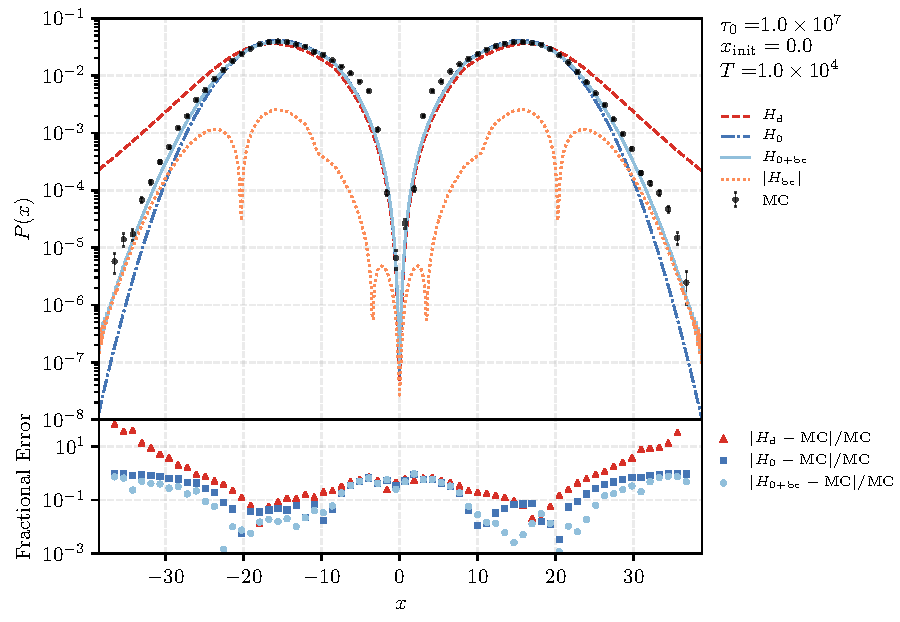
\includegraphics{1m_x_pdf_residualv2_log.pdf}
    \caption{Analytic solution for the outgoing spectrum compared with Monte Carlo at an optical depth of $1 \times 10^7$. It is evident that the solution $H_{\rm d}$ derived by \citet{1973MNRAS.162...43H} diverges significantly from the Monte Carlo simulations in the line wings. The $H_{\rm bc}$ correction term, when added to the solution $H_0$ derived by \citet{2006ApJ...649...14D}, results in an overall smaller fractional deviation from the Monte Carlo and a much closer match to the Monte Carlo in the wing.}
    \label{fig:sol_mc_residual}
\end{figure}

% Discussion of various solutions compared with Monte Carlo
[Brief discussion of Monte Carlo runs to set up comparison]

In Fig. \ref{fig:sol_mc_residual}, the contribution of the flux from Eq. \ref{eq:Hbc} is examined alongside the solutions $H_{\rm d}$ and $H_{\rm 0}$. We find that $H_{\rm 0 + bc} = H_{\rm 0} + H_{\rm bc}$ has considerably lower fractional error with the Monte Carlo in the line wing.

\section{ time-dependent diffusion }

In order to understand the wait time distribution, the time-dependent response to an impulse is found. For simplicity a $J=0$ boundary condition will be used. This is expected to be a good approximation for $\tau_0 \gg 1$. 

The source is changed to the form
\be
j_{\rm em} & = & \frac{E}{4\pi} \delta^3(\vec{x} - \vec{x}_s) \delta(\nu-\nu_{\rm s})\delta (t) .
\label{eq:jem2}
\ee
where $E$ is the energy emitted in the impulse at time $t=0$. 
The resulting equation for $J(r,\sigma,t)$ is
\be
-3 \frac{k\phi}{c} \frac{\partial J}{\partial t} + \nabla^2 J + \left( \frac{k}{\Delta} \right)^2 \frac{\partial^2 J}{\partial \sigma^2}
& = & - \frac{\sqrt{6} kE}{4\pi \Delta^2} \delta(\vec{x}) \delta (\sigma - \sigma_s ) \delta (t).
\label{eq:diffusion_eqn}
\ee
The coefficient of $\partial J/\partial t$ has explicit dependence on $\sigma$. Separation of variables may be achieved in Equation \ref{eq:diffusion_eqn} by assuming an expansion in terms of spherical Bessel functions in $r$ and a Fourier expansion in time to find the form
\be
J(r,\sigma,t) & = & \sum_{n=1}^\infty \int_{-\infty}^\infty \frac{d\omega}{2\pi} J(n,\sigma,\omega) j_0(\kappa_n r) e^{-i \omega t},
\ee
where $\kappa_n = n\pi/R$ enforces the $J(R,\sigma,t)=0$ boundary condition and the spherical Bessel function is $j_0(x)=\sin(x)/x$. For the solution to be real requires that $J(n,\sigma,-\omega) = J^*(n,\sigma,\omega)$. The equation for $J(n,\sigma,\omega)$ becomes
\be
\frac{\partial^2 J}{\partial \sigma^2} & = & \left( \frac{\Delta \kappa_n}{k} \right)^2 J
- 3i\omega \frac{\Delta^2 \phi}{ck} J
- \sqrt{ \frac{3}{32} } \frac{E}{kR^3} n^2 \delta(\sigma - \sigma_s).
\label{eq:response}
\ee
The $\delta(\sigma - \sigma_s)$ enforces a discontinuity
\be
\frac{\partial J(n,\sigma_s^{(+)},\omega)}{\partial \sigma} - \frac{\partial J(n,\sigma_s^{(-)},\omega)}{\partial \sigma} & = & 
- \sqrt{ \frac{3}{32} } \frac{E}{kR^3} n^2
\label{eq:discontinuity}
\ee
and the boundary conditions are $J(n,\pm \infty,\omega)=0$. Since $\phi \propto \sigma^{-2/3}$, the solution at large $\sigma$ is 
\be
J(n,\sigma,\omega) & \propto & e^{-\kappa_n \Delta |\sigma| /k}
= e^{-\sqrt{\pi} n |\sigma | / \tau_0}.
\label{eq:finite_bc}
\ee

To solve the second order Equation \ref{eq:response}, starting points at large $\pm |\sigma|$ are chosen, and the dependence in Equation \ref{eq:finite_bc} is used for the starting slope. The solution is then integrated toward the singularity at $\sigma_s$ from each side. The two starting values are varied until $J(n,\sigma,\omega)$ is continuous at $\sigma_s$ and satisfies the desired jump in slope in Equation \ref{eq:discontinuity}. Since the solution is linear in the starting conditions, only two integrations with different starting values are necessary.



For small $t$ the solution is nearly a delta function in radius



    
\end{frame}


%\begin{figure}
%\plotone{KT_Eri.pdf}
%\caption{The Swift/XRT X-ray light curve for the first year after 
%outburst of the suspected recurrent nova KT Eri. At a maximum count rate of 
%328 ct/s, KT Eri was the brightest nova in X-rays observed to date. All 
%the component figures (6) are available in the Figure Set. Note that
%these components that are {\bf not} shown in the compiled pdf. The figure
%set consists of the same figures as shown in Figure \ref{fig:pyramid}. 
%The example figure shown for figure sets can be one component or many. 
%\label{fig:fig4}}
%\end{figure}



\acknowledgments




\appendix

\section{ derivation of the transfer equation }

\citet{1973MNRAS.162...43H} first showed that the transfer equation for the mean  intensity $J$ will satisfy a Poisson equation involving second derivatives of space and frequency variables. In this section we will briefly review the derivation of this equation including photon destruction terms and an emission term.

The radiative intensity $I = dE/(dA dt d\Omega d\nu)$ is the energy per perpendicular area $dA$, per time $dt$, per solid angle $d\Omega$ and per frequency $d\nu$ \citep{1986rpa..book.....R}. Here the time-dependence of $I$ has been ignored, which assumes the fluid is changing on timescales long compared to a light-crossing time. The intensity $I=I(\vec{x},\vec{n}, \nu)$ will be considered a function of position $\vec{x}$, photon (unit) direction vector $\vec{n}$, and cyclic frequency $\nu$. In the Eddington and two-stream approximations, $I(\vec{x},\nu) \simeq J(\vec{x},\nu) + 3 \vec{n} \cdot \vec{H}(\vec{x},\nu)$, where $J=(1/4\pi) \int d\Omega I$ is the mean intensity and $\vec{F} = 4\pi \vec{H}= \int d\Omega \vec{n} I$ is the flux.  

Photons of frequency $\nu$ near line center frequency $\nu_0$ are considered. The Doppler width will be written $\Delta = \nu_0 v_{\rm th}/c$, where $v_{\rm th}=\sqrt{2k_{\rm B}T/m_{\rm H}}$ is the thermal speed of hydrogen atoms of mass $m_{\rm H}$ and temperature $T$, and $c$ is the speed of light. The photon frequency in Doppler units will be written $x = (\nu-\nu_0)/\Delta$. For upper-state de-excitation rate $\Gamma$, the ratio of natural to Doppler broadening is $a=\Gamma/(4\pi \Delta)$. 
The transfer equation is \citep{1986rpa..book.....R}
\be
\frac{1}{c} \frac{\partial I}{\partial t} + \vec{n} \cdot \grad I & =& - \left( \alpha_{\rm sc} + \alpha_{\rm abs} \right) I + (1-p) j_{\rm sc} + j_{\rm em}.
\label{eq:rteqn}
\ee
The scattering coefficient, or inverse mean free path to scattering, is 
\be
\alpha_{\rm sc} & = & n_{\rm sc}\, \frac{\pi e^2}{m_e c}\, f\, \frac{H(x,a)}{\sqrt{\pi} \Delta}
= k \phi   
\ee
where $n_{\rm sc}$ is the number density of scatterers, $e$ and $m_e$ have their usual meaning, $f$ is the oscillator strength of the transition, $H(x,a)$ is the Voigt function, $k = n_{\rm sc} (\pi e^2/m_e c) f$, and the Voigt line profile is $\phi = H(x,a)/(\sqrt{\pi} \Delta)$, which is normalized as $\int d\nu\, \phi(\nu) = 1$. The absorption coefficient $\alpha_{\rm abs}$, or inverse mean free path to true absorption, is a sum over number density of the absorber times absorption cross section. Once the incoming photon has promoted the electron to an excited state, the collisional de-excitation probability is $p$, and hence only a fraction $1-p$ of the excitations lead to re-emission of photons. ``Hummer Case II-b"  \citep{1962MNRAS.125...21H} will be used for the redistribution function, for which the incoming photon is absorbed by the atom according to the natural broadening in the rest frame, re-emitted with a dipole phase function $g(\vec{n},\vec{n}^\prime)=(3/16\pi)(1+[\vec{n}\cdot \vec{n}^\prime]^2)$, which is appropriate for a 1s-2p transition \citep{1982qe}, and the result is averaged over a Maxwell-Boltzmann distribution of speeds for the atom. The result can be written
\be
j_{\rm sc}(\vec{x},\vec{n},\nu) & = & k \int \frac{ d^3v}{ \pi^{3/2} v_{\rm th}^3} e^{-v^2/v_{\rm th}^2}\, 
\int d\Omega^\prime \int d\nu^\prime \,
g(\vec{n},\vec{n}^\prime) 
\nonumber \\ & \times & 
\delta \left( \nu - \nu^\prime - \nu_0 \vec{v} \cdot (\vec{n}-\vec{n}^\prime)/c \right)
\left( \frac{\Gamma/4\pi^2}{ \left(\nu^\prime - \nu_0 - \nu_0 \vec{v} \cdot \vec{n}^\prime/c \right)^2 + (\Gamma/4\pi)^2 } \right)  \,
I(\vec{x},\vec{n}^\prime,\nu^\prime)
\nonumber \\ & = & 4\pi k \int d\Omega^\prime \int d\nu^\prime R(\vec{n},\nu; \vec{n}^\prime,\nu^\prime) I(\vec{x},\vec{n}^\prime,\nu^\prime),
\ee
which defines the Case II-b redistribution function
\be
R(\vec{n},\nu; \vec{n}^\prime,\nu^\prime) & = & \frac{ g(\vec{n},\vec{n}^\prime) }{ 4\pi }
\int \frac{ d^3v}{ \pi^{3/2} v_{\rm th}^3} e^{-v^2/v_{\rm th}^2}\,
\delta \left( \nu - \nu^\prime - \nu_0 \vec{v} \cdot (\vec{n}-\vec{n}^\prime)/c \right)
\left( \frac{\Gamma/4\pi^2}{ \left(\nu^\prime - \nu_0 - \nu_0 \vec{v} \cdot \vec{n}^\prime/c \right)^2 + (\Gamma/4\pi)^2 } \right)
\ee
found in \citet{1962MNRAS.125...21H}.


The integral of the redistribution function over outgoing and incoming frequency are
\be
\int d\nu\ R(\vec{n},\nu; \vec{n}^\prime,\nu^\prime) 
& = & \frac{1}{4\pi} g(\vec{n},\vec{n}^\prime) \phi(\nu^\prime)
\ee 
and
\be
\int d\nu^\prime \ R(\vec{n},\nu; \vec{n}^\prime,\nu^\prime) 
& = & \frac{1}{4\pi} g(\vec{n},\vec{n}^\prime) \phi(\nu)
\ee 
where the right hand side is the usual Voigt function, the thermal average of the Lorentzian. The former result implies that the integrated source and sink terms for scattering cancel for $p=1$. In addition, $d\nu d\Omega 4\pi R(\vec{n},\nu; \vec{n}^\prime,\nu^\prime)/\phi(\nu^\prime) $ is the normalized distribution for the outgoing $\vec{n}$ and $\nu$ given the incoming $\vec{n}^\prime$ and $\nu^\prime$. 

This probability distribution can be used to define the moments of the frequency shift
\be
\langle \Delta \nu^n \rangle & = & \frac{ \int d\nu^\prime R (\nu-\nu^\prime)^n}{\int d\nu^\prime R}
= \frac{1}{\phi(\nu)}
\int \frac{ d^3v}{ \pi^{3/2} v_{\rm th}^3} e^{-v^2/v_{\rm th}^2}\,
\left( \frac{\nu_0 \vec{v} \cdot (\vec{n}-\vec{n}^\prime) }{c} \right)^n
\left( \frac{\Gamma/4\pi^2}{ \left(\nu - \nu_0 - \nu_0 \vec{v} \cdot \vec{n}/c \right)^2 + (\Gamma/4\pi)^2 } \right),
\ee
which are functions of $\nu$, $\vec{n}$ and $\vec{n}^\prime$. These integrals can be evaluated in terms of the dimensionless moments of the parallel velocity distribution, defined as
\be
\langle u_\parallel^n \rangle(x,a) & = & \frac{a/\pi }{H(x,a)} \int 
\frac{du_\parallel u_\parallel^n e^{-u_\parallel^2}  }{(x-u_\parallel)^2 + a^2}.
\ee
The end results for the first and second moments are
\be
\langle \Delta \nu \rangle & = & \Delta \langle u_\parallel \rangle \left( 1 - \vec{n} \cdot \vec{n}^\prime \right)
\\
\langle \Delta \nu^2 \rangle & = & \Delta^2 
\left[ \langle u_\parallel^2 \rangle
\left( 1 - \vec{n} \cdot \vec{n}^\prime \right)^2
+ \frac{1}{2} \left( 1 - \left( \vec{n} \cdot \vec{n}^\prime\right)^2 \right) \right].
\ee

For small frequency shifts $\nu-\nu^\prime$, the incoming intensity may be expanded as 
\be
I(\vec{x},\vec{n}^\prime,\nu^\prime) & \simeq  &
I(\vec{x},\vec{n}^\prime,\nu) 
+ 
\frac{\partial I(\vec{x},\vec{n}^\prime,\nu)}{\partial \nu }(\nu^\prime-\nu)
+ \frac{1}{2} \frac{\partial^2 I(\vec{x},\vec{n}^\prime,\nu)}{\partial \nu^2} (\nu^\prime-\nu)^2 + ...
\ee 
and the Fokker-Planck expansion of $j_{\rm sc}$ is
\be
j_{\rm sc}(\vec{x},\vec{n},\nu) & \simeq  & 4\pi k \int d\Omega^\prime \int d\nu^\prime R(\vec{n},\nu; \vec{n}^\prime,\nu^\prime) 
\left[ 
I(\vec{x},\vec{n}^\prime,\nu) + \frac{\partial I(\vec{x},\vec{n}^\prime,\nu)}{\partial \nu }(\nu^\prime-\nu)
+ \frac{1}{2} \frac{\partial^2 I(\vec{x},\vec{n}^\prime,\nu)}{\partial \nu^2 }(\nu^\prime-\nu)^2
\right]
\nonumber \\ 
& =& 
k\phi(\nu) \int d\Omega^\prime g 
\left[ 
I(\vec{x},\vec{n}^\prime,\nu) 
- \frac{\partial I(\vec{x},\vec{n}^\prime,\nu)}{\partial \nu }
\langle \Delta \nu \rangle
+ \frac{1}{2} \frac{\partial^2 I(\vec{x},\vec{n}^\prime,\nu)}{\partial \nu^2 }
\langle \Delta \nu^2 \rangle
\right]
\ee 
To perform the angular integrals, the Eddington approximation for the angular dependence is inserted with the following result
\be
j_{\rm sc} & = & k\phi J - k\phi \Delta \langle u_\parallel \rangle \left( \frac{\partial J}{\partial \nu} - \frac{6}{5} \vec{n} \cdot \frac{\partial \vec{H}}{\partial \nu} \right)
+ \frac{1}{2} \Delta^2 k\phi \left[ 
\frac{\partial^2 J}{\partial \nu^2} \left( \frac{7}{5} \langle u_\parallel^2 \rangle + \frac{3}{10} \right)
- \frac{12}{5} \langle u_\parallel^2 \rangle 
\vec{n} \cdot \frac{\partial^2 \vec{H}}{\partial \nu^2} \right]
\nonumber \\ & \simeq & 
k\phi J - k\phi \Delta \langle u_\parallel \rangle  \frac{\partial J}{\partial \nu} 
+ \frac{1}{2} \Delta^2 k\phi \left( \frac{7}{5} \langle u_\parallel^2 \rangle + \frac{3}{10} \right)
\frac{\partial^2 J}{\partial \nu^2} .
\label{eq:jsc}
\ee
The first term in Equation \ref{eq:jsc}, $k\phi J$, represents re-emission of the photon through de-excitation of the atom. It cancels the $-k\phi J$ term in Equation \ref{eq:rteqn} that corresponds to excitation of the atom. The terms involvingfrequency derivatives of $\vec{H}$, if carried through the calculation,end up giving terms smaller than then largest terms by a factor of $1/x^2$, which is small on the line wing. These terms are ignored from here on.

If only scattering is included, the transfer equation becomes
\be
\frac{1}{c} \frac{\partial }{\partial t} \left( J + 3\vec{n} \cdot \vec{H} \right)
+ \vec{n} \cdot \grad \left( J + 3\vec{n} \cdot \vec{H} \right)
& = & - k\phi \Delta \langle u_\parallel \rangle  \frac{\partial J}{\partial \nu} 
+ \frac{1}{2} \Delta^2 k\phi \left( \frac{7}{5} \langle u_\parallel^2 \rangle + \frac{3}{10} \right)
\frac{\partial^2 J}{\partial \nu^2}.
\ee
Integrating over angle and frequency then gives
\be
\frac{1}{c} \frac{\partial J(\vec{x}) }{\partial t} +  \grad \cdot \vec{H}(\vec{x}) & = & \int d\nu
\left( - k\phi \Delta \langle u_\parallel \rangle  \frac{\partial J}{\partial \nu} 
+ \frac{1}{2} \Delta^2 k\phi \left( \frac{7}{5} \langle u_\parallel^2 \rangle + \frac{3}{10} \right)
\frac{\partial^2 J}{\partial \nu^2}
\right) 
\nonumber \\ & =& 
k \int d\nu J \frac{\partial }{\partial \nu} 
\left( \phi \Delta \langle u_\parallel \rangle
+ \frac{\partial }{\partial \nu}\left[ \frac{1}{2} \phi \Delta^2 
\left( \frac{7}{5} \langle u_\parallel^2 \rangle + \frac{3}{10}  \right) \right]
\right) = 0,
\ee
where $\vec{H}(\vec{x})$ is the frequency integrated flux, and $\grad \cdot \vec{H}(\vec{x})  = 0 $ if there are no sources or sinks of radiation. Integration by parts has been used to factor $J$ out, assuming each term goes to zero at infinity. The quantity inside brackets must be constant, and since each term should go to zero at infinity, that constant is zero. Hence the first and second moments of the frequency shift are related by
\be
\phi \Delta \langle u_\parallel \rangle
& = & -  \frac{\partial }{\partial \nu}\left[ \frac{1}{2} \phi \Delta^2 
\left( \frac{7}{5} \langle u_\parallel^2 \rangle + \frac{3}{10}  \right) 
\right].
\ee
As an example, on the damping wing, $\phi \simeq a/(\pi x^2)$, $\langle u_\parallel \rangle \simeq 1/x$ and $\langle u_\parallel^2 \rangle \simeq 1/2$, and this identity is satisfied. The redistribution function can then be rewritten
\be
j_{\rm sc} & \simeq & k\phi J + \frac{1}{2} k \Delta^2 \frac{\partial }{\partial \nu} 
\left[ \phi  \left( \frac{7}{5} \langle u_\parallel^2 \rangle + \frac{3}{10}  \right)\frac{\partial J}{\partial \nu}  \right]
\simeq k\phi J + \frac{1}{2} k \Delta^2 \frac{\partial }{\partial \nu} 
\left( \phi \frac{\partial J}{\partial \nu}  \right)
\ee
where the last equality (see e.g. \citealt{1994ApJ...427..603R}) is valid on the damping wing where $\langle u_\parallel^2 \rangle \simeq 1/2$.
The following equations will use the approximations for the damping wing.

Thus far the transfer equation is
\be
\frac{1}{c} \frac{\partial }{\partial t} \left( J + 3\vec{n} \cdot \vec{H} \right) + \vec{n} \cdot \grad \left( J + 3 \vec{n} \cdot \vec{H} \right)
& =& j_{\rm em}
- \left( k\phi + \alpha_{\rm abs} \right) \left( J + 3 \vec{n} \cdot \vec{H} \right)
+
(1-p) \left[
k\phi J + \frac{1}{2} k \Delta^2 \frac{\partial }{\partial \nu} 
\left( \phi \frac{\partial J}{\partial \nu}  \right)
\right]
\nonumber \\ & \simeq & 
j_{\rm em} - 3k\phi \vec{n} \cdot \vec{H} - \left( p k\phi  + \alpha_{\rm abs} \right) J 
+ \frac{1}{2} k \Delta^2 \frac{\partial }{\partial \nu} 
\left( \phi \frac{\partial J}{\partial \nu}  \right),
\label{eq:rteqn2}
\ee
where leading order dissipative terms were kept in the second equality.
The moment equations are
\be
\frac{1}{c} \frac{\partial J}{\partial t} + \grad \cdot \vec{H} & = & j_{\rm em} 
- \left(p k\phi +  \alpha_{\rm abs} \right) J
+ \frac{1}{2} k \Delta^2 \frac{\partial }{\partial \nu} 
\left( \phi \frac{\partial J}{\partial \nu}  \right)
\ee
and
\be
\frac{1}{c} \frac{\partial \vec{H}}{\partial t} + \frac{1}{3} \grad J & =& - \left( k \phi + \alpha_{\rm abs} \right) \vec{H}.
\ee
The $\partial \vec{H}/\partial t$ term may be dropped for slowly changing sources.
Assuming the coefficients are constant in space, these two equations can be combined together to find
\be
\frac{1}{c} \frac{\partial J}{\partial t} - \frac{1}{3 (k\phi + \alpha_{\rm abs})} \nabla^2 J
& =& j_{\rm em} 
- \left( p k\phi +  \alpha_{\rm abs} \right) J
+ \frac{1}{2} k \Delta^2 \frac{\partial }{\partial \nu} 
\left( \phi \frac{\partial J}{\partial \nu}  \right).
\ee
Making the change of variables to $d\sigma = \sqrt{2/3}d\nu/(\Delta^2 \phi)$, the equation can be rewritten in the standard form \citep{1973MNRAS.162...43H}
\be
-3 \left( \frac{k\phi + \alpha_{\rm abs}}{c}\right) \frac{\partial J}{\partial t} + \nabla^2 J + \left( \frac{k}{\Delta} \right)^2 \left( 1 + \frac{\alpha_{\rm abs}}{k\phi} \right)\frac{\partial^2 J}{\partial \sigma^2} & = & 
-3 \left( k\phi + \alpha_{\rm abs}\right) j_{\rm em}
+ 3 \left( k\phi + \alpha_{\rm abs}\right) \left( pk\phi + \alpha_{\rm abs}\right) J.
\label{eq:finaleqn}
\ee
    
For emission with luminosity $L$, with a delta function in space $\delta^3(\vec{x} - \vec{x}_s)$ at source position $\vec{x}_s$, a delta function in frequency $\delta(\nu-\nu_{\rm s})$ at source frequency $\nu_{\rm s}$, and isotropic in angles, the emission coefficient is
\be
j_{\rm em} & = & \frac{L}{4\pi} \delta^3(\vec{x} - \vec{x}_s) \delta(\nu-\nu_{\rm s}).
\label{eq:jem}
\ee
Multiplying by a factor $-3k\phi$, as appears in Equation \ref{eq:finaleqn}, the delta function in $\nu$ becomes a delta function in $\sigma$ of the form
\be
-3k\phi j_{\rm em}  &= & - \frac{ \sqrt{6} kL}{4\pi \Delta^2} \delta^3(\vec{x} - \vec{x}_s) \delta (\sigma - \sigma_{\rm s}),
\label{eq:jem_v2}
\ee
where $\sigma_s = \sigma(\nu_s)$. 




\bibliography{ref.bib}{}
\bibliographystyle{aasjournal}



\end{document}

